%% LyX 2.3.6.1 created this file.  For more info, see http://www.lyx.org/.
%% Do not edit unless you really know what you are doing.
\documentclass[english]{article}
\usepackage[T1]{fontenc}
\usepackage[latin9]{inputenc}
\usepackage{url}
\usepackage{amsmath}
\usepackage{graphicx}

\makeatletter

%%%%%%%%%%%%%%%%%%%%%%%%%%%%%% LyX specific LaTeX commands.
%% Because html converters don't know tabularnewline
\providecommand{\tabularnewline}{\\}

%%%%%%%%%%%%%%%%%%%%%%%%%%%%%% Textclass specific LaTeX commands.
\newenvironment{lyxcode}
	{\par\begin{list}{}{
		\setlength{\rightmargin}{\leftmargin}
		\setlength{\listparindent}{0pt}% needed for AMS classes
		\raggedright
		\setlength{\itemsep}{0pt}
		\setlength{\parsep}{0pt}
		\normalfont\ttfamily}%
	 \item[]}
	{\end{list}}

\makeatother

\usepackage{babel}
\begin{document}
\title{Prediction of Covid-19 cases using constructed features by Grammatical
Evolution}
\author{Ioannis G. Tsoulos$^{(1)}$\thanks{Corresponding author. Email: itsoulos@uoi.gr},
Alexandros Tzallas$^{(1)}$, Dimitrios Tsalikakis$^{(2)}$}
\date{$^{(1)}$Department of Informatics and Telecommunications, University
of Ioannina, 47100 Arta, Greece \\
$^{(2)}$University of Western Macedonia, Department of Engineering
Informatics and Telecommunications, Greece}
\maketitle
\begin{abstract}
A widely used method that constructs features with the incorporation
of the so - called Grammatical Evolution is proposed here to predict
the Covid-19 cases as well as the mortality rate. The method creates
new artificial features from the original ones using a Genetic algorithm
and is guided by a BNF grammar.\textbf{ }After the artificial features
are generated, the original data set is modified based on these features
and an artificial neural network is applied to the modified data and
the results are reported. From the comparative experiments done, it
was clear that feature construction has an advantage over other machine
learning methods for predicting pandemic elements.\\
\textbf{Keywords:} Genetic algorithms; feature construction; Covid-19
pandemic; stochastic methods; Grammatical Evolution
\end{abstract}

\section{Introduction }

The world changed in December 2019, when the first reports emerged
of a mysterious infection in the Chinese province, Wuhan. Subsequently,
the WHO\textbf{ (}World Health Organization) declared a new global
pandemic on March 11, 2020. The name given to the new coronavirus
was SARS-CoV-2 (Severe Acute Respiratory Syndrome) and the name given
to the corresponding disease was Covid-19.\textbf{ }As Andersen mentioned
\cite{Andersen}, the virus's origin is natural selection in an animal
host before the zoonotic transfer or natural selection in humans following
the zoonotic transfer.\textbf{ }At the time of writing, the number
of diagnosed cases of Covid-19 was about 650.000.000 and the number
of people who had died was over 6.500.000. So the fatality rate was
about 1\%, although this rate may be lower since many people have
fallen ill without undergoing any diagnostic test. 

Due to the seriousness of the topic, since the beginning of the pandemic
until now, a multitude of publications have appeared in the relevant
literature on this topic and many of them use computational techniques
to predict the course of the disease. For example, Wang \cite{Wang}
used the Patient Information Based Algorithm (PIBA), that uses real
- time data collected from patients in Wuhan. With this data, he wrote
an algorithm to forecast the death rates. Also, Tomar and Gupta \cite{Gupta},
used Long Short-Term Memory (LSTM) to predict the number of COVID-19
cases. Zhang et al\cite{Zhang} used a Poisson model to analyze the
Covid-19 cases in Canada,France,Germany, Italy, UK and USA. Pinter
et al. \cite{Pinter} used an ANFIS system and a multilayered perceptron-
imperialist competitive algorithm (MLP-ICA) to predict the mortality
rate for Hungary.\textbf{ }Smith et al. \cite{Smith}, used machine
learning techniques for a dataset made of blood samples taken from
Covid-19 patients from a hospital in the region of Wuhan, in order
to estimate the mortality rate.\textbf{ }Additionally, papers \cite{mask1,mask2}
using machine learning techniques to recognize faces behind masks
has emerged in recent years.

The current work utilizes a feature construction method initially
presented in \cite{fcmain}, to predict the Covid-19 cases and deaths
for a series of randomly selected countries. The method is based on
Grammatical Evolution \cite{gemain} and creates artificial features
from the original ones without a priory knowledge of the structure
of the problem. The method has been used with success in a series
of scientific fields such as Spam identification \cite{fc1}, Fetal
heart classification \cite{fc2}, epileptic oscillations \cite{fcmain}
etc. Also, recently a software that implements the feature construction
method using modern programming approaches has been published \cite{qfc}.
In the case of the Covid-19 data, the only feature is the recording
time in ascending form and the output is the number of cases or deaths
for that recording. The proposed method creates 1-3 artificial features
from the recording time and, subsequently an artificial neural network
\cite{neural1,neural2} is trained on the modified data. The experimental
results are compared against other methods used to train neural networks
and the proposed technique appears to significantly outperform the
others in terms of accuracy.

The rest of this article is organized as follows: in section \ref{sec:Method-description}
the main aspects of Grammatical Evolution and the steps of the proposed
technique are outlined in detail, in section \ref{sec:Experimental-results}
the experimental results are outlined and finally in section \ref{sec:Conclusions}
some conclusions and guidelines for the extension of the proposed
technique are listed.

\section{Method description \label{sec:Method-description}}

The proposed technique is divided into two phases. During the first
phase, artificial new features are created from the original ones
using Grammatical Evolution and a Genetic Algorithm. The new features
are evaluated using a Radial Basis Function (RBF) network \cite{rbf1}
with $H$ processing units. The RBF network is selected as the evaluator
because the training procedure of RBF is much faster than those of
artificial neural networks. Subsequently, in the second phase, the
original dataset is transformed using the best located features and
a Genetic Algorithm is used to train a neural network on the modified
dataset.

\subsection{Grammatical Evolution\label{subsec:Grammatical-Evolution}}

Grammatical evolution is an evolutionary approach, where the chromosomes
are random numbers standing for production rules of a given BNF (Backus-Naur
form) grammar \cite{bnf1}. The Grammatical Evolution was initially
used for regression \cite{ge_program1,ge_program2} and to solve trigonometric
identities \cite{ge_trig}, but it has been applied in a variety of
scientific fields, such as automatic composition of music \cite{ge_music},
neural network construction \cite{ge_nn,ge_nn2}, automatic constant
creation \cite{ge_constant}, evolution of video games \cite{ge_pacman,ge_supermario},
energy demand estimation \cite{ge_energy}, combinatorial optimization
\cite{ge_comb}, cryptography \cite{ge_crypt} etc. The BNF grammar
is defined as the set \textbf{$G=\left(N,T,S,P\right)$ }with:
\begin{itemize}
\item \textbf{$N$ }is the set of the non - terminal symbols, used to produce
series of terminal symbols through production rules.
\item \textbf{$T$ }is the set of terminal symbols of the grammar. For example,
terminal symbols could be the digits in an arithmetic expression of
the operators.
\item \textbf{$S$ }is the starting non - terminal symbol of the grammar.
The production of a valid expression initiates from this symbol.
\item \textbf{$P$ }is the set of production rules. Every rule is in the
form \textbf{$A\rightarrow a$ }or\textbf{ $A\rightarrow aB,\ A,B\in N,\ a\in T$.}
\end{itemize}
The original grammar is expanded in Grammatical Evolution, with the
addition of a sequence number for each production rule.\textbf{ }The
chromosomes in Grammatical Evolution are integer numbers representing
sequence numbers of production rules. Subsequently, the production
procedure starts from the start symbol of the grammar and produces
valid programs by replacing non - terminal symbols with the right
hand of the selected production rule. The selection of the rule has
two steps: 
\begin{enumerate}
\item Retrieve the next element from the given chromosome and denote it
as $V$. 
\item The next production rule $R$ is calculated by 
\[
R=V\ \mbox{MOD}\ K
\]
where $K$ is the total number of production rules for the current
non - terminal symbol.
\end{enumerate}
In the current work the extend BNF grammar is illustrated in Figure
\ref{fig:BNF-grammar-of}. The non - terminal symbols are enclosed
in the symbols < > and the number N denotes the number of original
features. For the Covid-19 case the N is considered as 1. An example
of producing a valid expression is shown in the Table \ref{tab:table_with_steps}.
The chromosome is $x=\left[9,8,6,4,16,10,17,23,8,14\right]$ and $N=3$.
The valid expression created finally is\textbf{ $f(x)=x_{2}+\cos\left(x_{3}\right)$}. 

Considering the above mapping procedure, the steps to produce $N_{f}$
artificial features for a given chromosome $g$ are:
\begin{enumerate}
\item Divide the into $N_{f}$ parts. Each part $g_{i},\ i=1,..,N_{f}$
will construct a separate feature.
\item A feature $t_{i}$ is constructed for every $g_{i}$ using the grammar
given in Figure \ref{fig:BNF-grammar-of}
\item Construct a mapping function \textbf{
\begin{equation}
\mbox{FC}(\overrightarrow{x},g)=\left(t_{1}\left(\overrightarrow{x},g_{1}\right),t_{2}\left(\overrightarrow{x},g_{2}\right),\ldots,t_{N_{f}}\left(\overrightarrow{x},g_{N_{f}}\right)\right)\label{eq:mapping}
\end{equation}
}with $\overrightarrow{x}$ being the pattern from the original set.
\end{enumerate}
\begin{figure}
\caption{BNF grammar of the proposed method.\label{fig:BNF-grammar-of}}

\begin{lyxcode}
S::=<expr>~~~(0)~

<expr>~::=~~(<expr>~<op>~<expr>)~~(0)~~~~~~~~~~~~~

~~~~~~~~~~~|~<func>~(~<expr>~)~~~~(1)~~~~~~~~~~~~~

~~~~~~~~~~~|<terminal>~~~~~~~~~~~~(2)~

<op>~::=~~~~~+~~~~~~(0)~~~~~~~~~~~~~

~~~~~~~~~~~|~-~~~~~~(1)~~~~~~~~~~~~~

~~~~~~~~~~~|~{*}~~~~~~(2)~~~~~~~~~~~~~

~~~~~~~~~~~|~/~~~~~~(3)

<func>~::=~~~sin~~(0)~~~~~~~~~~~~~

~~~~~~~~~~~|~cos~~(1)~~~~~~~~~~~~~

~~~~~~~~~~~|exp~~~(2)~~~~~~~~~~~~~

~~~~~~~~~~~|log~~~(3)

<terminal>::=<xlist>~~~~~~~~~~~~~~~~(0)~~~~~~~~~~~~~~~~~~~~~~

~~~~~~~~~~~|<digitlist>.<digitlist>~(1)

<xlist>::=x1~~~~(0)~~~~~~~~~~~~~~

~~~~~~~~~~~|~x2~(1)~~~~~~~~~~~~~~

~~~~~~~~~~~\dots \dots \dots{}~~~~~~~~~~~~~

~~~~~~~~~~~|~xN~(N)

<digitlist>::=<digit>~~~~~~~~~~~~~~~~~~(0)~~~~~~~~~~~~~~~~~

~~~~~~~~~~~|~<digit><digit>~~~~~~~~~~~~(1)

~~~~~~~~~~~|~<digit><digit><digit>~~~~~(2)

<digit>~~::=~0~(0)~~~~~~~~~~~~~

~~~~~~~~~~~|~1~(1)~~~~~~~~~~~~~

~~~~~~~~~~~|~2~(2)~~~~~~~~~~~~~

~~~~~~~~~~~|~3~(3)~~~~~~~~~~~~~

~~~~~~~~~~~|~4~(4)~~~~~~~~~~~~~

~~~~~~~~~~~|~5~(5)~~~~~~~~~~~~~

~~~~~~~~~~~|~6~(6)~~~~~~~~~~~~~

~~~~~~~~~~~|~7~(7)~~~~~~~~~~~~~

~~~~~~~~~~~|~8~(8)~~~~~~~~~~~~~

~~~~~~~~~~~|~9~(9)
\end{lyxcode}
\end{figure}
\begin{table}
\caption{Steps to produce a valid expression from the BNF grammar.\label{tab:table_with_steps}}

\begin{tabular}{|c|c|c|}
\hline 
String & Chromosome & Operation\tabularnewline
\hline 
\hline 
<expr> & 9,8,6,4,16,10,17,23,8,14 & $9\mod3=0$\tabularnewline
\hline 
(<expr><op><expr>) & 8,6,4,16,10,17,23,8,14 & $8\mod3=2$\tabularnewline
\hline 
(<terminal><op><expr>) & 6,4,16,10,17,23,8,14 & $6\mod2=0$\tabularnewline
\hline 
(<xlist><op><expr>) & 4,16,10,17,23,8,14 & $4\mod3=1$\tabularnewline
\hline 
(x2<op><expr>) & 16,10,17,23,8,14 & $16\mod4=0$\tabularnewline
\hline 
(x2+<expr>) & 10,17,23,8,14 & $10\mod3=1$\tabularnewline
\hline 
(x2+<func>(<expr>)) & 17,23,8,14 & $17\mod4=1$\tabularnewline
\hline 
(x2+cos(<expr>)) & 23,8,14 & $23\mod2=1$\tabularnewline
\hline 
(x2+cos(<terminal>)) & 8,14 & $8\mod2=0$\tabularnewline
\hline 
(x2+cos(<xlist>)) & 14 & $14\mod3=2$\tabularnewline
\hline 
(x2+cos(x3)) &  & \tabularnewline
\hline 
\end{tabular}
\end{table}


\subsection{Feature creation step }

In this step a genetic algorithm in conjunction with the mapping procedure
of subsection \ref{subsec:Grammatical-Evolution} is used to produce
artificial features. The fitness function of the genetic algorithm
is the training error of an RBF neural network with $H$ processing
units. The steps are the following:
\begin{enumerate}
\item \textbf{Initialization step}

\begin{enumerate}
\item \textbf{Set} iter=0, the current number of generations.
\item \textbf{Consider} the set $\mbox{TR}=\left\{ \left(\overrightarrow{x_{1}},y_{1}\right),\left(\overrightarrow{x_{2}},y_{2}\right),\ldots,\left(\overrightarrow{x_{M}},y_{M}\right)\right\} $,
the original training set.
\item \textbf{Set} $N_{c}$ the number of chromosomes in the genetic population.
\item \textbf{Set} $N_{f}$ the number of constructed features. 
\item \textbf{Initialize} randomly in range $[0,255]$ every element of
each chromosome.
\item \textbf{Set} $N_{g}$ as the maximum number of generations.
\item \textbf{Set} $p_{s}\in[0,1]$ as the selection rate.
\item \textbf{Set} as $p_{m}\in[0,1]$ the mutation rate.
\end{enumerate}
\item \textbf{Termination check step.} \textbf{If} iter>=$N_{g}$ terminate.
\label{enu:Termination-check.-If}
\item \textbf{Calculate} the fitness $f_{i}$ of every chromosome $g_{i}$
with the following procedure:\label{enu:Calculate-the-corresponding-1}

\begin{enumerate}
\item \textbf{Create $N_{f}$ }features using the mapping procedure of subsection
\ref{subsec:Grammatical-Evolution}.
\item \textbf{Construct} the mapped training set 
\begin{equation}
\mbox{TN}=\left\{ \left(\mbox{FC}\left(\overrightarrow{x_{1}},g_{i}\right),y_{1}\right),\left(\mbox{FC}\left(\overrightarrow{x_{2}},g_{i}\right),y_{2}\right),\ldots,\left(\mbox{FC}\left(\overrightarrow{x_{M}},g_{i}\right),y_{M}\right)\right\} 
\end{equation}
 
\item \textbf{Train} an RBF neural network $C$ with $H$ processing units
on the new set $\mbox{TN }$ and obtain the following train error
\begin{equation}
E_{i}=\sum_{j=1}^{M}\left(C\left(\mbox{FC}\left(\overrightarrow{x_{j}},Z_{i}\right)\right)-y_{j}\right)^{2}
\end{equation}
\item \textbf{Set} $f_{i}=E_{i}$
\end{enumerate}
\item \textbf{Genetic Operators}

\begin{enumerate}
\item \textbf{Selection procedure: }The chromosomes are sorted according
to their fitness. The best $p_{s}\times N_{c}$ are copied intact
to the next generation.\textbf{ }The genetic operations of crossover
and mutation are applied to rest of the chromosomes.
\item \textbf{Crossover procedure:} During this process $\left(1-p_{s}\right)\times N_{c}$
offsprings will be created. For every couple of produced offsrpings,
two parents $(z,w)$ are selected using the well - known procedure
of tournament selection.\textbf{ }For every pair $(z,w)$ of parents,
two offsprings $\tilde{z}$ and $\tilde{w}$ are produced through
one point crossover. An example of one point crossover is shown in
Figure .
\item \textbf{Mutation procedure: }For each element of every chromosome
a random number $r\in\left[0,1\right]$ is produced. Subsequently
we change randomly the corresponding element if $r\le p_{m}$.
\end{enumerate}
\item \textbf{Set} iter=iter+1 and \textbf{goto} Step \ref{enu:Termination-check.-If}.
\end{enumerate}
\begin{figure}

\caption{An example of one point crossover. A randomly selected point is chosen
and the two subparts of the parents are exchanged.\label{fig:onepoint}}

\centering{}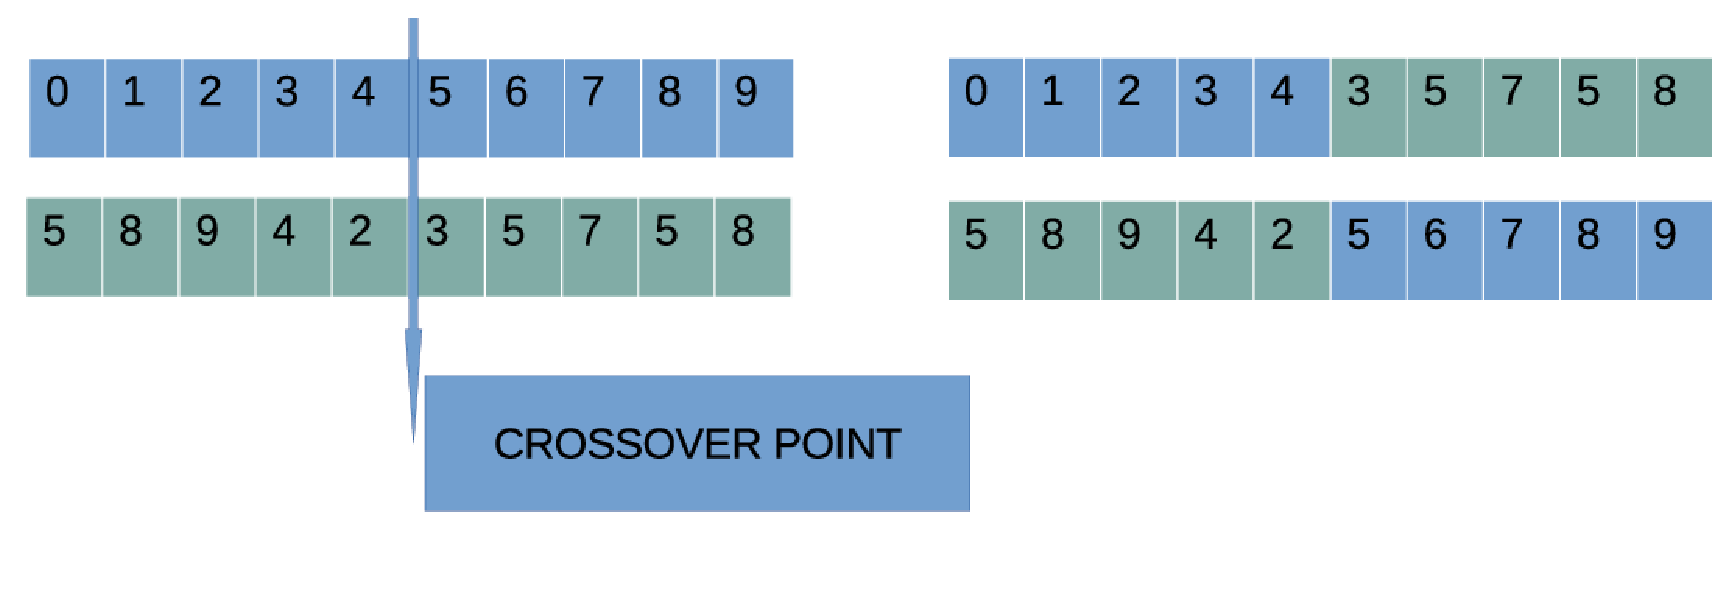
\includegraphics[scale=0.5]{onepoint_crossover}
\end{figure}


\subsection{Feature evaluation step}

During this step, the best chromosome $g_{b}$ of the first step is
obtained and used to create the modified train set 
\[
\mbox{TN}=\left\{ \left(\mbox{FC}\left(\overrightarrow{x_{1}},g_{b}\right),y_{1}\right),\left(\mbox{FC}\left(\overrightarrow{x_{2}},g_{b}\right),y_{2}\right),\ldots,\left(\mbox{FC}\left(\overrightarrow{x_{M}},g_{b}\right),y_{M}\right)\right\} 
\]
Afterwards a genetic algorithm is used to train an artificial neural
network with $H$ hidden nodes for this dataset. The neural network
used here is defined as a function $N\left(x,w\right)$, where $w$
is the weight vector to be estimated through the genetic algorithm
after the minimization of the following training error: 
\begin{equation}
E\left(N\left(x,w\right)\right)=\sum_{i=1}^{M}\left(N\left(\mbox{FC}\left(x_{i},g_{b}\right),w\right)-y_{i}\right)^{2}\label{eq:trainError}
\end{equation}
The neural network has a form also used in \cite{nnc}.\textbf{ }If
the neural network has one processing level, every output of each
hidden node is in the form:\textbf{
\begin{equation}
o_{i}(x)=\sigma\left(p_{i}^{T}x+\theta_{i}\right),\label{eq:eq1-1}
\end{equation}
}where $p_{i}$ is the weight vector and \textbf{$\theta_{i}$ }is
considered as the bias for output \textbf{$i.$ }The function $\sigma(x)$
is the well - known sigmoid function given by: \textbf{
\begin{equation}
\sigma(x)=\frac{1}{1+\exp(-x)}\label{eq:sig}
\end{equation}
}For a neural network with $H$ hidden nodes the final output is given
by:\textbf{
\begin{equation}
N(x)=\sum_{i=1}^{H}v_{i}o_{i}(x),\label{eq:eq1-2}
\end{equation}
}where $v_{i}$ is the weight for hidden node $i$. Hence, if we use
one weight $w$ for hidden nodes and biases the following form could
be used for he neural network:\textbf{
\begin{equation}
N\left(\overrightarrow{x},\overrightarrow{w}\right)=\sum_{i=1}^{H}w_{(d+2)i-(d+1)}\sigma\left(\sum_{j=1}^{d}x_{j}w_{(d+2)i-(d+1)+j}+w_{(d+2)i}\right)\label{eq:nn}
\end{equation}
}The value $d$ the size of input vector $\overrightarrow{x}.$ Also,
the total number of parameters of vector $\overrightarrow{w}$ is
$(d+2)\times H$. The Genetic Algorithm used here, is a global optimization
technique\cite{genetic1,genetic2}, that has been applied with success
in many problems such as electromagnetic \cite{gen_app1}, combinatorial
problems \cite{gen_app2}, design of water distribution networks \cite{gen_app3}
etc. Also, it has been used to train artificial networks in some works
from the relevant literature \cite{geneticnn1,geneticnn2,geneticnn3}.
The steps of the genetic algorithm used in the second step of the
proposed method are the following:
\begin{enumerate}
\item \textbf{Initialization} step.
\begin{enumerate}
\item \textbf{Set} as $N_{c}$ the number of chromosomes that will participate.
\item \textbf{Set} as $N_{g},$the maximum number of allowed generations.
\item \textbf{Set} as $p_{m}$, the mutation rate.
\item \textbf{Set} as $p_{s},$ the selection rate.
\item \textbf{Set} $\epsilon$ a small positive number, i.e $\epsilon=10^{-8}$.
\item \textbf{Initialize} randomly the chromosomes $g_{i},\ i=1,...,N_{c}$
For the case of neural networks every element of each chromosome is
considered as a double precision number. Also, the size of each chromosome
is $(d+2)\times H.$
\item \textbf{Set} iter=0
\end{enumerate}
\item \textbf{Check} for termination\label{enu:Check-for-termination.}.
\begin{enumerate}
\item \textbf{Obtain} the best fitness 
\[
f^{*}=\min_{i\in\left[0\ldots N_{c}\right]}f_{i}
\]
\item \textbf{Terminate} if $\mbox{iter}\ge N_{g}$ OR $f^{*}\le\epsilon$
\end{enumerate}
\item \textbf{Calculate} fitness. 
\begin{enumerate}
\item \textbf{For} $i=1,\ldots,N_{c}$ \textbf{do}
\begin{enumerate}
\item \textbf{Create} a neural network using as parameter vector the chromosome
$g_{i}.$
\item \textbf{Calculate} the fitness value $f_{i}=f\left(g_{i}\right)$
using the equation \ref{eq:trainError}.
\end{enumerate}
\item \textbf{EndFor}
\end{enumerate}
\item \textbf{Application} of genetic operators.
\begin{enumerate}
\item \textbf{Selection} operation. During selection, the chromosomes are
classified according to their fitness. The first\textbf{ $p_{s}\times N_{c}$}
are copied without changes to the next generation of the population.
The rest will be replaced by chromosomes that will be produced at
the crossover.
\item \textbf{Crossover} operation. In the crossover operation, $p_{s}\times N_{c}$
chromosomes are produced. For every couple of produced offsrpings,
two parents $(z,w)$ are selected using tournament selection.\textbf{
}For every pair $(z,w)$ of parents, two offsprings $\tilde{z}$ and
$\tilde{w}$ are produced according to the following equations:\textbf{
\begin{eqnarray}
\tilde{z_{i}} & = & a_{i}z_{i}+\left(1-a_{i}\right)w_{i}\nonumber \\
\tilde{w_{i}} & = & a_{i}w_{i}+\left(1-a_{i}\right)z_{i}\label{eq:crossover_ali-1}
\end{eqnarray}
}where $a_{i}$ is a random number with the property $a_{i}\in[-0.5,1.5]$
\cite{kaeloAli}. 
\item \textbf{Mutation} operation. For each element of every chromosome
a random number $r\in\left[0,1\right]$ is produced and the element
is altered if $r\le p_{m}$
\item \textbf{Set} iter=iter+1
\end{enumerate}
\item \textbf{Goto} step \ref{enu:Check-for-termination.}.
\end{enumerate}

\section{Experimental results \label{sec:Experimental-results}}

The data was freely available from the URL \url{https://ourworldindata.org/explorers/coronavirus-data-explorer}
and was downloaded for the start of pandemic until September 10, 2022.
To enable the machine learning models to better fit the data, the
following fair normalization took place in every dataset
\begin{enumerate}
\item The number of cases was divided by $10^{5}$.
\item The number of deaths was divided by $10^{3}$.
\end{enumerate}
The following countries were selected for testing: Algeria, Argentina,
Australia, Brazil, Bulgaria, Canada, Germany, Greece, Egypt and Japan.
For every country, two distinct datasets was obtained from the COVID-19
database, one dataset for the number of cases in every day of the
pandemic and one dataset for the number of deaths in every day of
the pandemic. Every run was executed 30 times for every dataset and
averages were measured. The random number generator used was the drand48()
of the C programming language. The parameters for the proposed method
are listed in the Table \ref{tab:Experimental-parameters.}. The results
for the COVID-19 cases are shown in the Table \ref{tab:error_cases}
and the results for the COVID-19 deaths are illustrated in the Table
\ref{tab:table_deaths}. The columns in both tables have the following
meaning:
\begin{enumerate}
\item The column COUNTRY contains the name of the country.
\item The column ADAM stands for the Adam optimization method \cite{Adam}
used to train a neural network with 10 processing nodes. The ADAM
method is implemented in OptimLib and it is available from \url{https://github.com/kthohr/optim}. 
\item The column MLPPSO represents the results using a neural network trained
with the help of Particle Swarm Optimization method \cite{pso1,pso2}.
The number of PSO particles was set to $N_{c}$ and the maximum number
of allowed iterations was set to $N_{g}$. The value for this parameters
are shown in the Table \ref{tab:Experimental-parameters.}. Also,
a BFGS method \cite{powell} was applied to best particle of the swarm
when the PSO finishes, in order to enhance the results. 
\item The column MLPGEN stands for the results obtained by a neural network
with ten processing units, that is trained using a Genetic algorithm
\cite{genetic1,genetic2}. The parameters for this algorithm are listed
in the Table \ref{tab:Experimental-parameters.}. Also, the BFGS was
applied to the best chromosome after the termination of the genetic
algorithm.
\item The column FC1 stands for the results obtained by the proposed method
with one constructed feature $\left(N_{f}=1\right)$. 
\item The column FC2 stands for the results obtained by the proposed method
with two constructed features $\left(N_{f}=2\right)$.
\item The column FC3 stands for the results obtained by the proposed method
with three constructed features $\left(N_{f}=3\right)$.
\end{enumerate}
Also, in both tables, an additional row was added to indicate the
average error and is denoted by AVERAGE. This extra column is graphically
plotted in Figures \ref{fig:graph_cases} and \ref{fig:graph_deaths}
for cases prediction and deaths prediction respectively.

From the execution of the above experiments, it is clear in principle
that the efficiency of the methods depends to a great extent on the
country in question. In some countries the test error is high and
in others quite low. This is probably due to the different course
of the number of cases and the mortality rate in each country separately.
Also, the proposed method has higher accuracy than the other techniques
even if only one artificial feature is created. In fact, in some cases
of countries, the test error of the proposed technique is so low that
it is almost zero. Using more than one feature appears to drastically
reduce the error, although the reduction appears to be more significant
between one and two features and less when a third constructed feature
is added.

\begin{table}
\caption{Experimental parameters.\label{tab:Experimental-parameters.}}

\centering{}%
\begin{tabular}{|c|c|}
\hline 
PARAMETER & VALUE\tabularnewline
\hline 
\hline 
$N_{c}$ & 500\tabularnewline
\hline 
$N_{g}$ & 200\tabularnewline
\hline 
$H$ & 10\tabularnewline
\hline 
$p_{s}$ & 0.10\tabularnewline
\hline 
$p_{m}$ & 0.05\tabularnewline
\hline 
$\epsilon$ & $10^{-8}$\tabularnewline
\hline 
\end{tabular}
\end{table}
\begin{table}
\caption{Total test error for the prediction of COVID-19 cases.\label{tab:error_cases}}

\centering{}%
\begin{tabular}{|c|c|c|c|c|c|c|}
\hline 
COUNTRY & ADAM & MLPPSO & MLPGEN & FC1 & FC2 & FC3\tabularnewline
\hline 
\hline 
Algeria & 0.31 & 0.08 & 0.286 & 0.0025 & 0.0006 & 0.0002\tabularnewline
\hline 
Argentina & 178.60 & 21.03 & 69.20 & 3.21 & 0.81 & 0.91\tabularnewline
\hline 
Australia & 144.46 & 20.33 & 30.96 & 1.52 & 0.37 & 0.34\tabularnewline
\hline 
Brazil & 198.26 & 81.94 & 75.79 & 11.93 & 8.97 & 6.50\tabularnewline
\hline 
Bulgaria & 4.01 & 1.29 & 2.67 & 0.037 & 0.0098 & 0.01\tabularnewline
\hline 
Canada & 27.68 & 6.12 & 20.65 & 0.33 & 0.20 & 0.15\tabularnewline
\hline 
Germany & 274.34 & 135.15 & 92.50 & 25.05 & 25.11 & 14.36\tabularnewline
\hline 
Greece & 25.07 & 12.08 & 9.25 & 3.62 & 1.60 & 2.75\tabularnewline
\hline 
Egypt & 0.24 & 0.13 & 0.44 & 0.005 & 0.029 & 0.003\tabularnewline
\hline 
Japan & 271.11 & 95.56 & 75.76 & 8.92 & 2.15 & 1.82\tabularnewline
\hline 
\textbf{AVERAGE} & \textbf{112.41} & \textbf{37.37} & \textbf{37.75} & \textbf{5.46} & \textbf{3.92} & \textbf{2.68}\tabularnewline
\hline 
\end{tabular}
\end{table}
\begin{table}
\caption{Predicting deaths per country.\label{tab:table_deaths}}

\begin{centering}
\begin{tabular}{|c|c|c|c|c|c|c|}
\hline 
COUNTRY & ADAM & PSOGEN & MLPGEN & FC1 & FC2 & FC3\tabularnewline
\hline 
\hline 
Algeria & 0.40 & 0.15 & 0.66 & 0.009 & 0.002 & 0.002\tabularnewline
\hline 
Argentina & 18.50 & 19.70 & 25.81 & 2.03 & 1.35 & 1.70\tabularnewline
\hline 
Australia & 1.69 & 0.44 & 1.00 & 0.05 & 0.03 & 0.03\tabularnewline
\hline 
Brazil & 416.54 & 282.46 & 230.52 & 52.42 & 16.75 & 16.57\tabularnewline
\hline 
Bulgaria & 3.80 & 2.76 & 16.50 & 0.15 & 0.10 & 0.08\tabularnewline
\hline 
Canada & 9.12 & 4.78 & 18.12 & 0.27 & 0.15 & 0.15\tabularnewline
\hline 
Germany & 116.56 & 37.06 & 40.49 & 3.03 & 2.07 & 4.17\tabularnewline
\hline 
Greece & 3.29 & 2.97 & 2.86 & 0.74 & 0.08 & 0.07\tabularnewline
\hline 
Egypt & 2.57 & 0.79 & 8.88 & 0.07 & 0.03 & 0.02\tabularnewline
\hline 
Japan & 43.10 & 22.07 & 13.74 & 0.32 & 0.12 & 0.13\tabularnewline
\hline 
\textbf{AVERAGE} & \textbf{61.56} & \textbf{37.32} & \textbf{35.86} & \textbf{5.91} & \textbf{2.07} & \textbf{2.29}\tabularnewline
\hline 
\end{tabular}
\par\end{centering}
\end{table}
\begin{figure}
\caption{Graphical representation of average error for predicting COVID-19
cases.\label{fig:graph_cases}}

\centering{}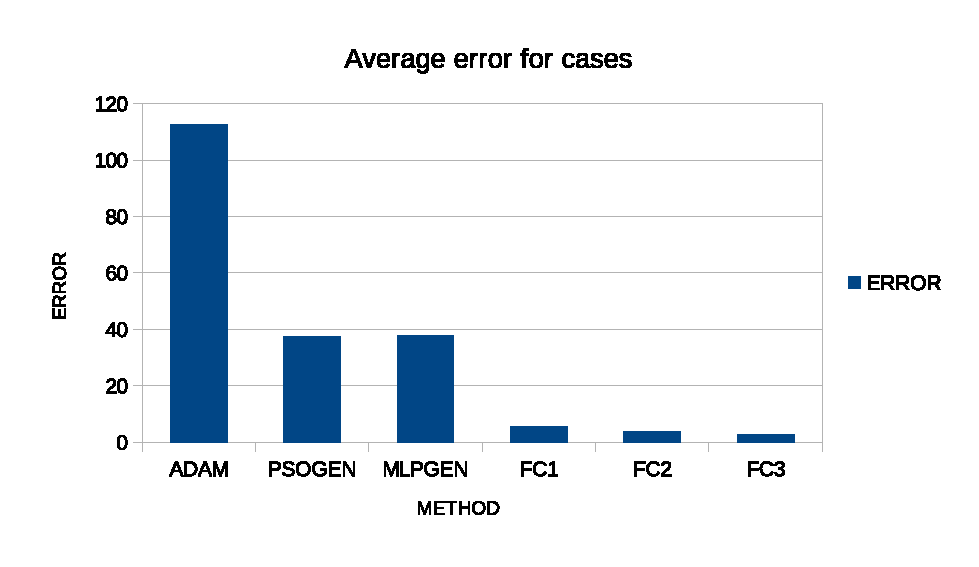
\includegraphics[scale=0.7]{covid19cases}
\end{figure}
\begin{figure}
\caption{Graphical representation of average error for predicting COVID-19
deaths.\label{fig:graph_deaths}}

\begin{centering}
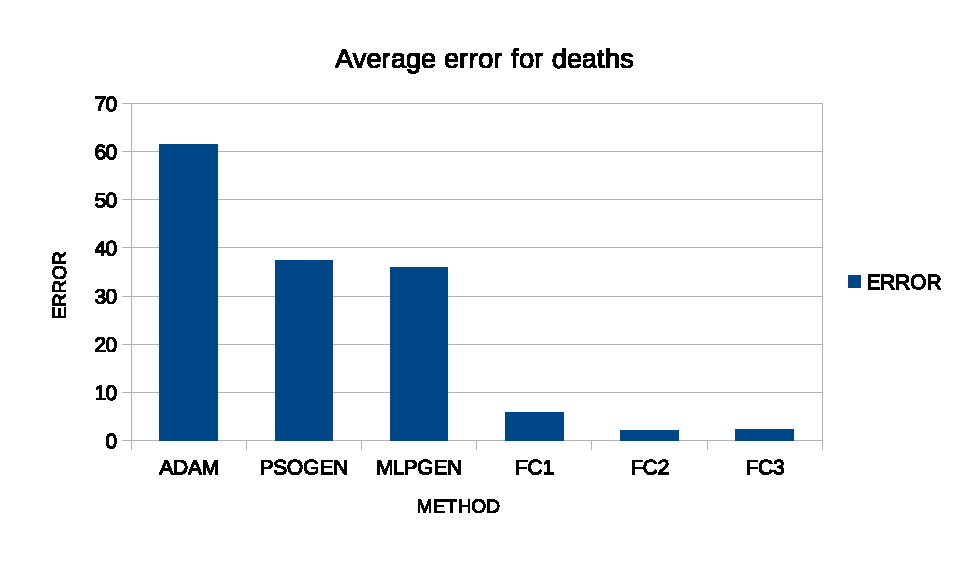
\includegraphics[scale=0.7]{deaths_figure}
\par\end{centering}
\end{figure}


\section{Conclusions\label{sec:Conclusions}}

An automated artificial feature construction method was presented
in this work to predict Covid-19 cases and deaths. The method is based
on Grammatical Evolution through two phases. In the first phase, 1-3
features were constructed using Genetic Algorithm and Grammatical
Evolution, and in the second phase, the new features were evaluated
by an artificial neural network trained using a Genetic Algorithm.
This procedure was applied to 10 randomly selected countries from
all continents and appeared to be significantly superior to other
techniques. Future improvements of the method may include:
\begin{enumerate}
\item Incorporation of more advanced stopping rules for the genetic algorithms
of the two phases.
\item Usage of another machine learning models instead of the RBF network
to evaluate the constructed features.
\item Usage of parallel techniques to speed up the feature creation process.
\item Use of the technique on data that will also contain demographic characteristics
of each country, in order to establish whether there is a correlation
of the rate of cases or mortality with any particular characteristic
of some countries.
\end{enumerate}
\begin{thebibliography}{10}
\bibitem{Andersen}K.G. Andersen, A. Rambaut, W.I. Lipkin, E.C. Holmes,
R.F. Garry, The proximal origin of sars-cov-2. Nature medicine \textbf{26},
pp. 450-452, 2020. 

\bibitem{Wang}L.Wang, J.Li, S.Guo, N.Xie, L.Yao, Y.Cao, S.W. Day,
S.C. Howard, J.C. Gra, T.Gu, et al. Real-time estimation and prediction
of mortality caused by covid-19 with patient information based algorithm.
Science of the Total Environment, page 138394, 2020.

\bibitem{Gupta}A.Tomar, N.Gupta, Prediction for the spread of covid-
19 in india and eectiveness of preventive measures. Science of The
Total Environment, page 138762, 2020.

\bibitem{Zhang}X.Zhang, R.Ma, L.Wang, Predicting turning point, duration
and attack rate of covid-19 outbreaks in major western countries.
Chaos, Solitons and Fractals, page 109829, 2020.

\bibitem{Pinter}G.Pinter, I.Felde, A.Mosavi, P. Ghamisi, R.Gloaguen,
Covid-19 pandemic prediction for hungary; a hybrid machine learning
approach. Mathematics, 8(6), 2020.

\bibitem{Smith}M.Smith, F. Alvarez, Identifying mortality factors
from machine learning using shapley values a case of covid19. Expert
Systems with Applications, 176:114832, 2021.

\bibitem{mask1}M.Loey, G.Manogaran, M.H.N. Taha, N.E.M. Khalifa,
A hybrid deep transfer learning model with machine learning methods
for face mask detection in the era of the covid-19 pandemic. Measurement,
167:108288, 2021.

\bibitem{mask2}I.Q.Mundial, M.S. Ul Hassan, M.I.Tiwana, W.S. Qureshi,
E.Alanazi, Towards facial recognition problem in covid-19 pandemic.
In 2020 4rd International Conference on Electrical, Telecommunication
and Computer Engineering (ELTICOM), pp. 210-214, 2020.

\bibitem{fcmain}D.Gavrilis, I.G. Tsoulos, E. Dermatas, Selecting
and constructing features using grammatical evolution, Pattern Recognition
Letters \textbf{29}, pp. 1358-1365, 2008.

\bibitem{gemain}M. O'Neill, C. Ryan, Grammatical evolution, IEEE
Transactions on Evolutionary Computation \textbf{5}, pp. 349-358,
2001.

\bibitem{fc1}D.Gavrilis, I.G. Tsoulos, E.Dermatas, Neural recognition
and genetic features selection for robust detection of e-mail spam.
In Hellenic Conference on Articial Intelligence, pp. 498-501. Springer,
2006.

\bibitem{fc2}G.Georgoulas, D.Gavrilis, I.G. Tsoulos, C.Stylios, J.Bernardes,
P.P. Groumpos, Novel approach for fetal heart rate classication introducing
grammatical evolution. Biomedical Signal Processing and Control \textbf{2},
pp.69-79, 2007.

\bibitem{fc3}O.Smart, I.G. Tsoulos, D.Gavrilis, G.Georgoulas, Grammatical
evolution for features of epileptic oscillations in clinical intracranial
electroencephalograms. Expert systems with applications \textbf{38},
pp.9991-9999, 2011.

\bibitem{qfc}I.G. Tsoulos, QFC: A Parallel Software Tool for Feature
Construction, Based on Grammatical Evolution, Algorithms \textbf{15},
295, 2022.

\bibitem{neural1}C. Bishop, Neural Networks for Pattern Recognition,
Oxford University Press, 1995.

\bibitem{neural2}G. Cybenko, Approximation by superpositions of a
sigmoidal function, Mathematics of Control Signals and Systems 2,
pp. 303-314, 1989.

\bibitem{rbf1}J. Park and I. W. Sandberg, Universal Approximation
Using Radial-Basis-Function Networks, Neural Computation\textbf{ 3},
pp. 246-257, 1991.

\bibitem{bnf1}J. W. Backus. The Syntax and Semantics of the Proposed
International Algebraic Language of the Zurich ACM-GAMM Conference.
Proceedings of the International Conference on Information Processing,
UNESCO, 1959, pp.125-132.

\bibitem{ge_program1}C. Ryan, J. Collins, M. O\textquoteright Neill,
Grammatical evolution: Evolving programs for an arbitrary language.
In: Banzhaf, W., Poli, R., Schoenauer, M., Fogarty, T.C. (eds) Genetic
Programming. EuroGP 1998. Lecture Notes in Computer Science, vol 1391.
Springer, Berlin, Heidelberg, 1998.

\bibitem{ge_program2}M. O\textquoteright Neill, M., C. Ryan, Evolving
Multi-line Compilable C Programs. In: Poli, R., Nordin, P., Langdon,
W.B., Fogarty, T.C. (eds) Genetic Programming. EuroGP 1999. Lecture
Notes in Computer Science, vol 1598. Springer, Berlin, Heidelberg,
1999.

\bibitem{ge_trig}C. Ryan, M. O\textquoteright Neill, J.J. Collins,
Grammatical evolution: Solving trigonometric identities, proceedings
of Mendel. Vol. 98. 1998.

\bibitem{ge_music}A.O. Puente, R. S. Alfonso, M. A. Moreno, Automatic
composition of music by means of grammatical evolution, In: APL '02:
Proceedings of the 2002 conference on APL: array processing languages:
lore, problems, and applications July 2002 Pages 148--155. 

\bibitem{ge_nn}L�dio Mauro Limade Campo, R. C�lio Lim� Oliveira,Mauro
Roisenberg, Optimization of neural networks through grammatical evolution
and a genetic algorithm, Expert Systems with Applications \textbf{56},
pp. 368-384, 2016.

\bibitem{ge_nn2}K. Soltanian, A. Ebnenasir, M. Afsharchi, Modular
Grammatical Evolution for the Generation of Artificial Neural Networks,
Evolutionary Computation \textbf{30}, pp 291--327, 2022.

\bibitem{ge_constant}I. Dempsey, M.O' Neill, A. Brabazon, Constant
creation in grammatical evolution, International Journal of Innovative
Computing and Applications \textbf{1} , pp 23--38, 2007.

\bibitem{ge_pacman}E. Galv�n-L�pez, J.M. Swafford, M. O\textquoteright Neill,
A. Brabazon, Evolving a Ms. PacMan Controller Using Grammatical Evolution.
In: , et al. Applications of Evolutionary Computation. EvoApplications
2010. Lecture Notes in Computer Science, vol 6024. Springer, Berlin,
Heidelberg, 2010.

\bibitem{ge_supermario}N. Shaker, M. Nicolau, G. N. Yannakakis, J.
Togelius, M. O'Neill, Evolving levels for Super Mario Bros using grammatical
evolution, 2012 IEEE Conference on Computational Intelligence and
Games (CIG), 2012, pp. 304-31.

\bibitem{ge_energy}D. Mart�nez-Rodr�guez, J. M. Colmenar, J. I. Hidalgo,
R.J. Villanueva Mic�, S. Salcedo-Sanz, Particle swarm grammatical
evolution for energy demand estimation, Energy Science and Engineering
\textbf{8}, pp. 1068-1079, 2020.

\bibitem{ge_comb}N. R. Sabar, M. Ayob, G. Kendall, R. Qu, Grammatical
Evolution Hyper-Heuristic for Combinatorial Optimization Problems,
IEEE Transactions on Evolutionary Computation \textbf{17}, pp. 840-861,
2013.

\bibitem{ge_crypt}C. Ryan, M. Kshirsagar, G. Vaidya, G. et al. Design
of a cryptographically secure pseudo random number generator with
grammatical evolution. Sci Rep \textbf{12}, 8602, 2022.

\bibitem{nnc}I.G. Tsoulos, D. Gavrilis, E. Glavas, Neural network
construction and training using grammatical evolution, Neurocomputing
\textbf{72}, pp. 269-277, 2008.

\bibitem{genetic1}D. Goldberg, Genetic Algorithms in Search, Optimization
and Machine Learning, Addison-Wesley Publishing Company, Reading,
Massachussets, 1989.

\bibitem{genetic2}Z. Michaelewicz, Genetic Algorithms + Data Structures
= Evolution Programs. Springer - Verlag, Berlin, 1996.

\bibitem{gen_app1}R.L. Haupt, An introduction to genetic algorithms
for electromagnetics, Antennas and Propagation Magazine 37, pp. 7-15,
1995.

\bibitem{gen_app2}J.J. Grefenstette, R. Gopal, B. J. Rosmaita, D.
Van Gucht, Genetic Algorithms for the Traveling Salesman Problem,
In: Proceedings of the 1st International Conference on Genetic Algorithms,
pp. 160 - 168, Lawrence Erlbaum Associates, 1985.

\bibitem{gen_app3}D. A. Savic, G. A. Walters, Genetic Algorithms
for Least-Cost Design of Water Distribution Networks, Journal of Water
Resources Planning and Management 123, pp. 67-77, 1997.

\bibitem{geneticnn1}F. H. F. Leung, H. K. Lam, S. H. Ling and P.
K. S. Tam, Tuning of the structure and parameters of a neural network
using an improved genetic algorithm, IEEE Transactions on Neural Networks
\textbf{14}, pp. 79-88, 2003.

\bibitem{geneticnn2}A. Sedki, D. Ouazar, E. El Mazoudi, Evolving
neural network using real coded genetic algorithm for daily rainfall--runoff
forecasting, Expert Systems with Applications \textbf{36}, pp. 4523-4527,
2009.

\bibitem{geneticnn3}A. Majdi, M. Beiki, Evolving neural network using
a genetic algorithm for predicting the deformation modulus of rock
masses, International Journal of Rock Mechanics and Mining Sciences
\textbf{47}, pp. 246-253, 2010.

\bibitem{kaeloAli}P. Kaelo, M.M. Ali, Integrated crossover rules
in real coded genetic algorithms, European Journal of Operational
Research \textbf{176}, pp. 60-76, 2007.

\bibitem{Adam}D. P. Kingma, J. L. Ba, ADAM: a method for stochastic
optimization, in: Proceedings of the 3rd International Conference
on Learning Representations (ICLR 2015), pp. 1--15, 2015.

\bibitem{pso1}J. Kennedy, R.C. Eberhart, The particle swarm: social
adaptation in information processing systems, in: D. Corne, M. Dorigo
and F. Glover (eds.), New ideas in Optimization, McGraw-Hill, Cambridge,
UK, pp. 11-32, 1999.

\bibitem{pso2}F. Marini, B. Walczak, Particle swarm optimization
(PSO). A tutorial, Chemometrics and Intelligent Laboratory Systems
\textbf{149}, pp. 153-165, 2015.

\bibitem{powell}M.J.D Powell, A Tolerant Algorithm for Linearly Constrained
Optimization Calculations, Mathematical Programming \textbf{45}, pp.
547-566, 1989. 
\end{thebibliography}

\end{document}
